\documentclass[12pt]{jarticle}
\usepackage{url}
\usepackage[dvipdfmx]{graphicx}
\usepackage{graphicx}
\begin{document}
\thispagestyle{empty}
\begin{center}
{\huge 2~0~2~6 年度~~卒~~業~~論~~文}
\vspace*{3.5cm}

{\LARGE\bf 個人の聴感特性に基づいて音楽を画像に変換する手法の研究} % ← 自分の研究テーマに置き換える
\vspace*{2cm}

{\large 2025年11月14日}  % ← 提出日
\vspace*{2cm}

{\large 情報科学科}

{\large （学籍番号：2022311042）}% ← 自分の学籍番号
\vspace*{3mm}

{\Large 神~野~~友~哉}  % ← 自分の名前
\vspace*{4cm}

{\large 愛知県立大学情報科学部}
\end{center}
\newpage 

% \setcounter{page}{1}

\section*{概要}
% 研究論文の内容について,500 - 600 字程度でまとめる.
% この概要を読めば,大体どういうことを研究したのかがわかるように書く.
% 具体的には,どういう問題について,どのような研究を行って,その結果どのような
% 結論が得られたか,というポイントについて簡潔にまとめる.

本研究は, 音楽をもとに視覚的イメージを自動生成する手法の開発を目的とする.
音楽が聴覚的情報であるのに対し, 視覚的表現との対応関係は明確に定義されていない.
そこで本研究では,音楽から得られる音響特徴量を中間表現として用い,これをテキスト情報に変換し,
最終的に画像を生成するシステムを構築した. 具体的には, まず楽曲からテンポ,スペクトル重心,
エネルギー量などの音響特徴量を抽出し, それらを入力としてニューラルネットワーク（NN）により
複数の単語ラベルを自動生成するモデルを構築した. このモデルにより,音楽の雰囲気や感情的印象を言語的に表現できるようにした.
次に,生成された単語群を昨今話題の生成 AI Chat GPT に入力し, 得られたテキストプロンプトを用いて画像生成AIにより視覚的イメージを生成した.
最後に, 元の音楽と生成された画像を被験者に提示し, 主観評価実験を通して両者の対応の自然さを検証した.
その結果, 多くの被験者の雰囲気の捉え方に類似傾向があることと, 音楽と生成された画像の雰囲気の合致度にバラつきあることが示された.
本手法が音楽と視覚表現の橋渡しとして, 様々な課題を残していることが判明した.

\newpage
\tableofcontents
\newpage

% 以下,章の名前は各自適当に変えてもよい

\section{はじめに}
% 研究の背景・動機・目的などを述べる.
音楽が聴き手に示す情報の大半は”音”と”名前”に限られているため,
記憶の中の"音"の情報だけを頼りに, 思い出したい音楽を探すと大変苦労した経験がある.
そのため, ”視覚”情報を追加できると印象を深められると考えた.

\subsection{研究の背景}
音楽をジャンルとしての単語に分類する研究は盛んに行われてきたが\cite{Xiaoli}\cite{Tzanetakis}\cite{Meyers},
音楽を中間材料としての単語に対応させてから画像生成を試みるという研究は,確認する限り全く無いものであった.
その為, 本研究では音楽から単語への変換及び, 単語から画像生成のプロセスにおける有効性があるか, 検証する必要があると考えられたのである。

\subsection{研究の目的}
% 研究の動機・目的については,上述した背景の下で,
% 自分がどのような問題意識の下で本研究を行おうとするのか,
% 研究の目的は何かといったことを記述する.
本研究では, 音楽の持つ情報を機械的に画像に対応させる
方法を検討し, 人間的な感性を伴った対応が実現可能かどうか
確かめることが目的である.

\subsection{本論文の構成}

% (書き方の例)

% 本論文では,人工知能のアルゴリズムについて研究を行う.
% 本論文の以下の構成は次のようになっている.
% 第２章では,本論文で使用する諸概念について述べる.
% 第３章では,人工知能の探索問題に対して,α-β-γ 法のアルゴリズムを提案し,
% 第４章では,提案されたアルゴリズムの評価を行う.
% 最後に,第５章で本論文の結論を述べる.
% なお,付録として α-β-γ アルゴリズムのプログラムと実行結果を加えた.
本論文では, 音楽から人間にとって適切だと思えるような画像を生成する方法について研究を行う.
本論文の以下の構成は次のようになっている.
第２章では, 準備として本論文で使用する諸概念について述べる.
第３章では, 音楽から中間表現としてのテキスト情報の対応及び外部の画像生成サイトを用いて生成する方法を提案し,
第４章では, 提案されたアルゴリズムの評価を行う.
最後に,第５章で本論文の結論を述べる.
なお,付録として 実行環境Google Colaboratoryでのpythonプログラムと学習データcsvファイル, 学習モデルを加えた.

\newpage 
\section{準備}  

% この論文で使う概念や用語の定義を説明する.
\addtolength{\leftskip}{3cm}
\begin{description}
  \item[特徴量 : ]データの特徴を数値化して, 機械学習などの分析で扱えるようにしたもの
  \item[ニューラルネットワーク(以降NNと称する) : ]人間の脳の神経細胞(ニューロン)の働きを模したコンピューターの数理モデル
  \item[教師あり学習 : ]正解ラベル付きのデータセット（入力featureと出力labelの対応がある）を用いてAIモデルを学習させる機械学習の手法
  \item[半教師あり学習 : ]少量のラベル付きデータと,大量のラベルなしデータの両方を使用して機械学習モデルを訓練する手法
  \item[活性化関数 : ]NNの各ニューロンにおいて, 入力値から出力値に変換する関数
  \item[シグモイド関数 : ]いかなる実数入力であっても0から1の間の値に変換する関数であり, 機械学習の二値分類で確率を出力したい際に用いられる 
\end{description}
\addtolength{\leftskip}{-3cm}

\newpage
\section{本論}
\subsection{問題提起} 

% 本研究で対象とする問題は何かを説明する.
音楽は聴覚を通じて人に感情や雰囲気を想起させる表現媒体であるが,
その印象は数値や明確な言語として表現することが難しい.
一方で, 近年発展が著しい画像生成AIは, 主にテキスト情報を入力としており,
音楽のような非言語的, 感覚的情報を直接扱うことは困難である.
また, 音楽をジャンルや感情語に分類する研究は数多く存在するものの,
音楽の雰囲気を中間的な単語表現に変換し, 
その単語を用いて画像生成を行う手法については十分に検討されていない.
さらに, 音楽の受け取り方には個人差が存在するにもかかわらず,
個人の聴感特性を考慮した音楽と視覚表現の対応に関する研究は少ない.
そこで本研究では, 
音楽から抽出される特徴量を基に雰囲気を表す単語を生成し,
その単語を用いて画像を生成することが可能かどうか.
また, その結果が人間の主観的印象とどの程度一致するか, 聴感特性に個人差がどの程度あるかを明らかにすることを課題とする.

\subsection{研究の説明}
% 上記問題に対して,本研究ではどのような手法により,
% どう問題を解いたのかを説明する.
% 本研究の技術的課題として, NN の学習データの水増し,
% 画像生成に用いるラベル(単語)の妥当性, ならびに生成ラベル(単語)の情報量という三点を設定する.
% また, 個人の聴感特性は, 音楽から生成ラベル(単語)に変換する際の NN の学習で十分再現可能か確かめ,
% それから ChatGPT が画像を生成可能かどうかも検証する.
% 示した問題に対して順に, 半教師あり学習の導入, 筆者による暫定的なラベル(単語)設定, そしてラベル(単語)間の同時生成頻度に基づく間引きを行った.
% 加えて, 個人の聴感特性については, 生成された画像がおおよそ私個人の趣旨に合うと感じているため,  NN が私の感性を学習していると見なせるはずである.
% 音楽から得られた生成ラベル(単語)は, 画像を生成するように命令された生成 AI ChatGPT に入力され画像を生成する.
% 音楽の雰囲気と合致している度合いを尋ねた客観的な評価結果を, 以下のアンケートに示す.
本研究では, 音楽から視覚的イメージを生成するために, 音楽データを数値的特徴量へ変換し,
その特徴量から音楽の雰囲気を表す単語ラベルを生成する手法を用いた.
本節では, 使用した音楽データセット, 特徴量抽出方法, および単語生成モデルについて説明する.

\subsubsection{音楽データセット}

本研究では, 音楽ジャンル分類の分野で広く用いられている GTZAN データセットを使用した.
GTZAN データセットは, 10 ジャンルから構成され, 各ジャンルにつき 100 曲，合計 1000 曲の音楽データを含む.
各楽曲は約 30 秒の音源であり, 本研究ではこれらを学習および評価用データとして利用した.

\subsubsection{音響特徴量の抽出}

音楽の雰囲気を数値的に表現するため, 各楽曲から以下の音響特徴量を抽出した.
Zero Crossing Rate は波形がゼロを跨ぐ頻度を表し, 音の高さや速さに関係する特徴量である.
Spectral Centroid は周波数軸上の重心を示し, 音の明るさやバランスを表現する指標である.
Root Mean Square（RMS）は信号の二乗平均平方根であり, 経時的な音の大きさを表す.
Spectral Bandwidth は周波数成分の広がりを示し, 音の豪華さや厚みを反映する.
Tempo は 1 分間あたりのビート数を表し, 楽曲の速さを示す指標である.
Spectral Flatness はスペクトルの平坦さを示し, 音がノイズ的か単音的かを判別する特徴量である.
Spectral Contrast は周波数帯域におけるピークと谷の差を表し, 音の鋭さや明瞭さを示す.
Mel-Frequency Cepstral Coefficients（MFCC）は, 人間の聴覚特性を考慮した周波数尺度に基づく特徴量であり, 音楽信号の特徴を表現するために広く用いられている.
本研究では, Spectral Contrast を 7 次元, MFCC の平均値および標準偏差を合計 26 次元, その他の特徴量を 6 次元として抽出し, 合計 39 次元の音響特徴量を得た.

\subsubsection{単語ラベル生成モデル}

抽出した 39 次元の音響特徴量を入力として, 音楽の雰囲気を表す単語ラベルを生成するモデルを構築した.
本研究では，浅層ニューラルネットワークを用い, 出力層にシグモイド関数を適用することで,
複数の単語ラベルを同時に出力可能な マルチラベル分類を実現した.
シグモイド関数を用いることで, 各単語ラベルが付与される確率を独立に推定でき,
音楽が複数の雰囲気を同時に持つ場合にも対応可能となる. モデルの構成を図Xに示す, 
生成された単語ラベルは, 画像生成を行う生成AIに入力され, 音楽の雰囲気に基づいた視覚的イメージの生成に利用される.

\subsubsection{画像生成用プロンプトの生成}

前節で生成された単語ラベルは, そのまま画像生成AIに入力するのではなく, 画像生成に適した形式へと整理した.
本研究では, 単語ラベルを意味的なカテゴリごとに分類し, 各カテゴリ内で出力確率の高い単語を選択する方法を用いた.
具体的には, 形容詞カテゴリから上位 2 語, 情景を表す名詞カテゴリから上位 2 語, 
色カテゴリから上位 1 語, 季節カテゴリから上位 1 語を選択した. 
これは, 名詞:構図, 形容詞:雰囲気, 色:視覚的統一感, 季節:時間的文脈として十分な情報を含有すると考察したためである。
そうして選択された単語は, 確率の高い順に連結し, 画像生成AIに入力するテキストプロンプトとして使用した. 
このような選択規則により, プロンプトが過度に冗長になることを防ぎつつ, 音楽の雰囲気を多面的に表現することが可能となった.
さらに, 画像生成AIに対しては, 単語列挙型のプロンプトとして解釈されるよう, あらかじめ共通の指示文（プロンプト命令）を付与した.
\begin{quote}
以降、単語を複数列挙するのでそれで絵を描いてもらいます。
各々の絵はそれまでの絵との関連はないようにしたい
\end{quote}
この指示文では, 以降に列挙される単語群のみを手掛かりとして 1 枚の画像を生成すること, および各画像生成がそれ以前の生成結果と
意味的な関連を持たないようにすることを明示した. 
実際のプロンプトはこの指示文に続けて, 前述の規則により選択された単語ラベルを空白区切りで記述する形式とした. 
以下に, 生成に用いたプロンプトの一例を示す.
\begin{quote}
暗く寂しい 冬 神秘的な場所 自然風景 青 幻想的・夢幻的
\end{quote}
上記プロンプトを入力して生成された画像を, 図\ref{fig:generated_images}(a) に示す.
\begin{quote}
都市・人工物 高貴・荘厳 静か・滑らか 秋 時間・空模様 茶色
\end{quote}
同様に, 図\ref{fig:generated_images}(b) に示す. 

\begin{figure}[htbp]
  \centering
  \begin{minipage}{0.48\textwidth}
    \centering
    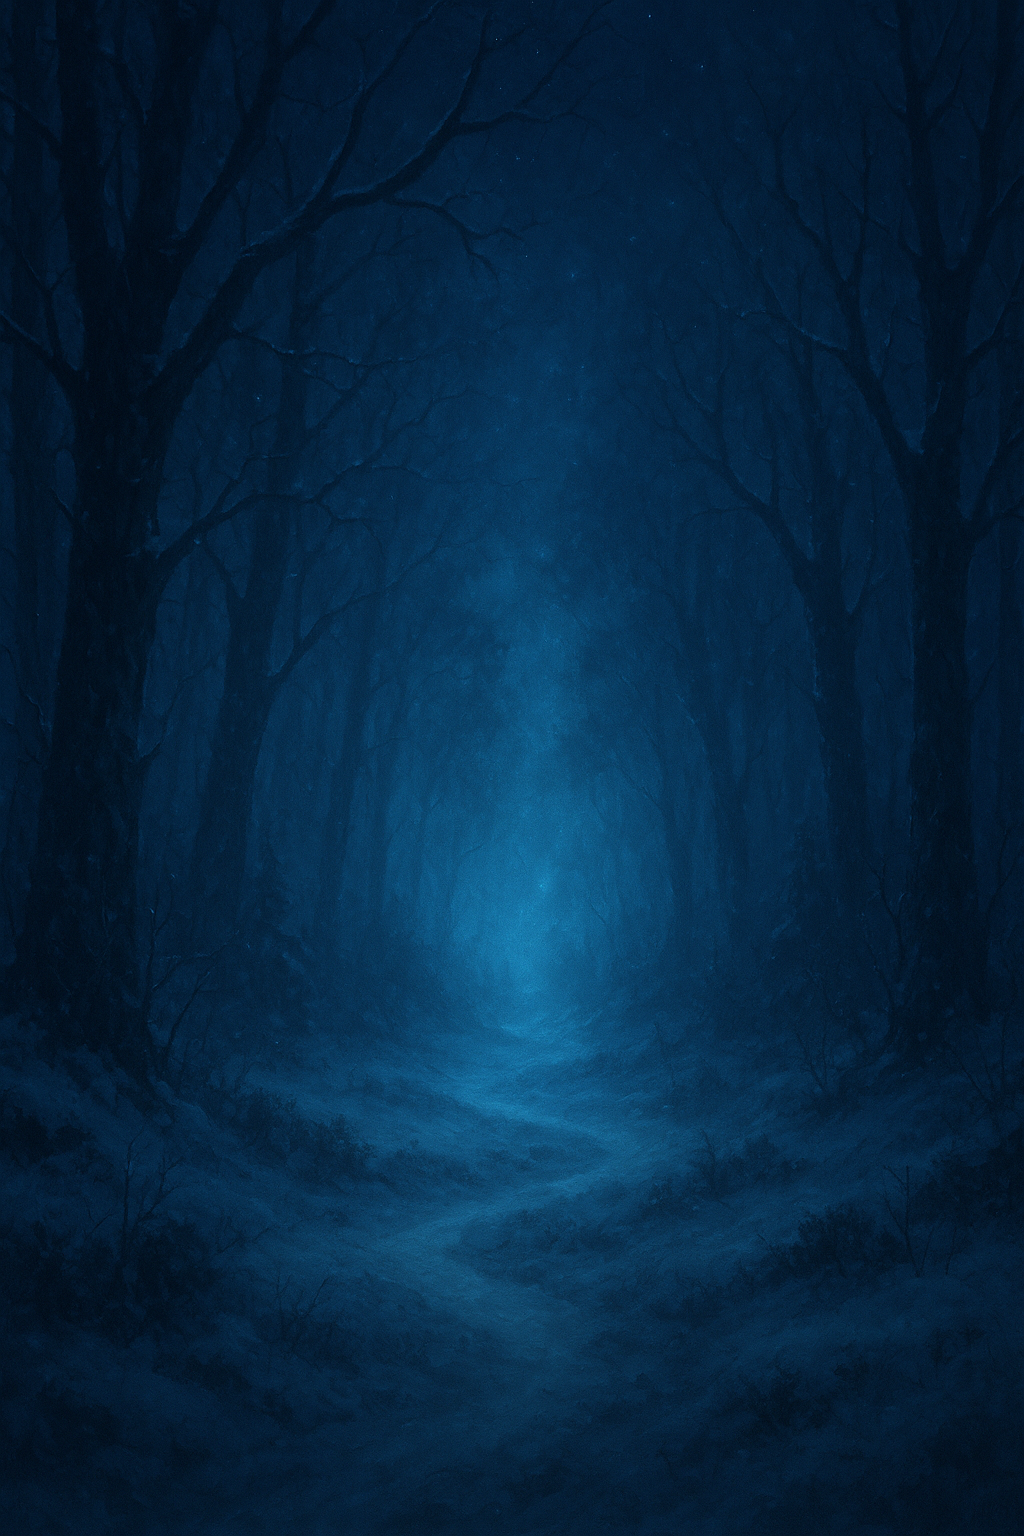
\includegraphics[width=0.3\textwidth]{./画像/seisei1.png}
    \caption*{(a) 楽曲Aから生成された画像}
  \end{minipage}
  \hfill
  \begin{minipage}{0.48\textwidth}
    \centering
    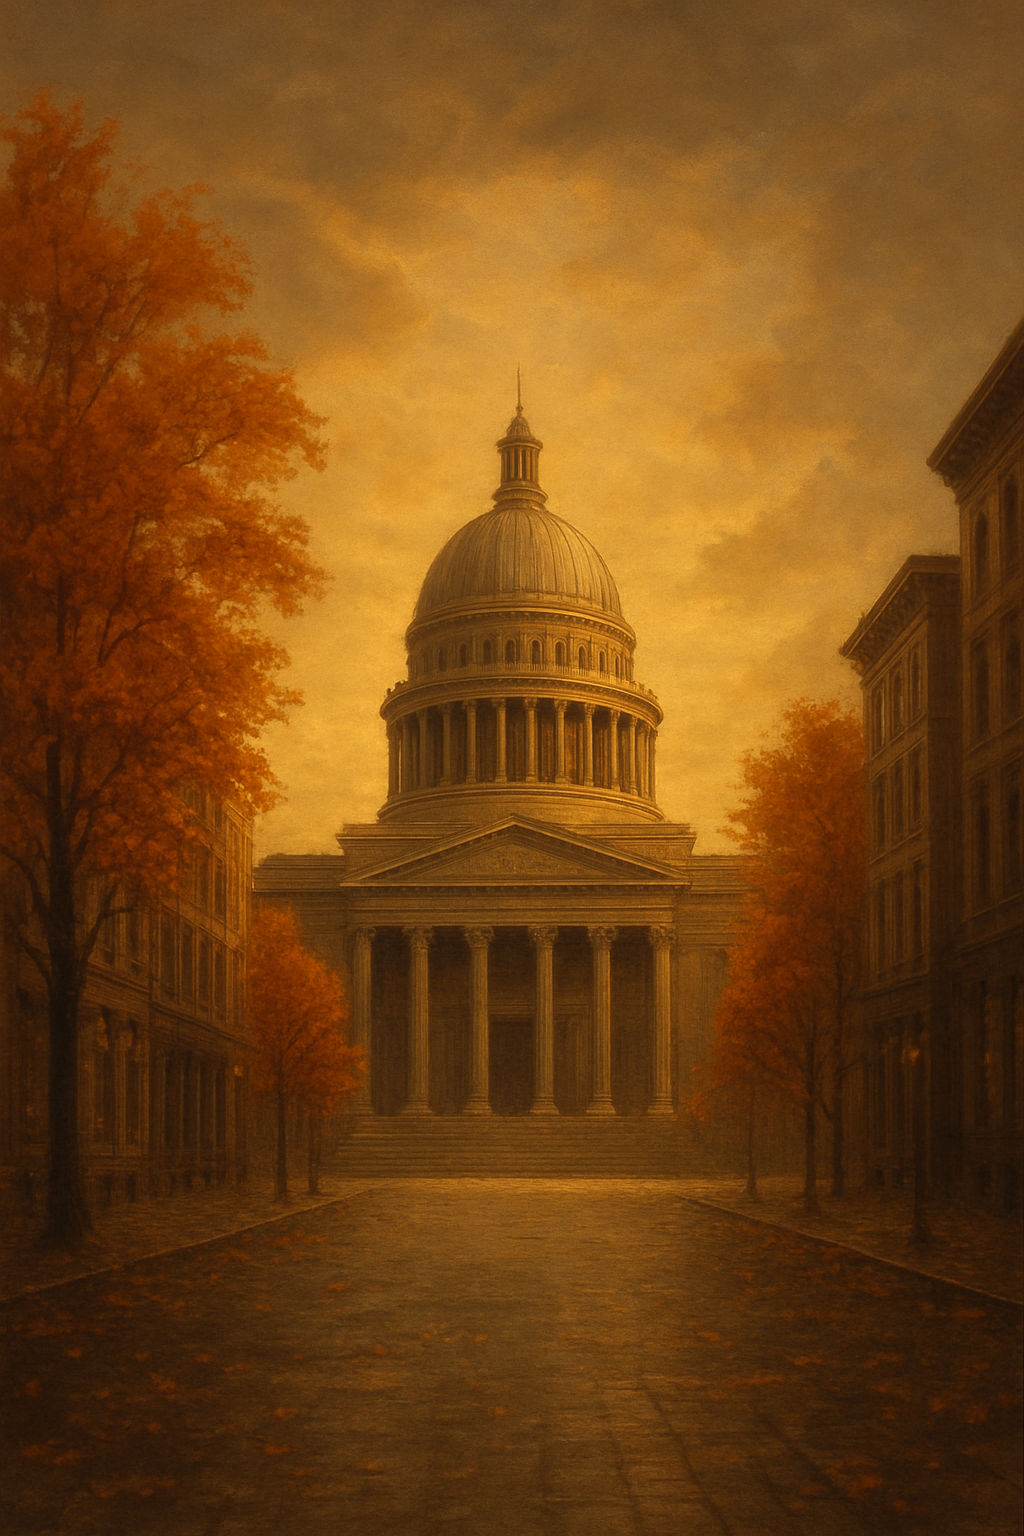
\includegraphics[width=0.3\textwidth]{./画像/seisei2.png}
    \caption*{(b) 楽曲Bから生成された画像}
  \end{minipage}
  \caption{音楽から生成された単語ラベルに基づき生成された画像例}
  \label{fig:generated_images}
\end{figure}

このように, プロンプトの文法構造を固定し, 単語ラベルのみを変化させることで, 
生成される画像の差異が音楽から生成された単語に起因するよう配慮した. 

\subsection{音楽と生成画像の雰囲気の合致アンケート結果}

本アンケートは, 音楽と生成画像の雰囲気の合致度について評価することを目的として実施した.
評価は 0 から 10 の 11 段階尺度を用い, 
0 を「雰囲気が全く異なる」, 10 を「雰囲気が完全に一致している」と定義した. 
被験者数は N=5 とし, 回答は匿名で収集した. 
図\ref{fig:questionnaire_results}に, 
音楽と生成画像の雰囲気の一致度に関するアンケート結果を示す.

\begin{figure}[htbp]
  \centering
  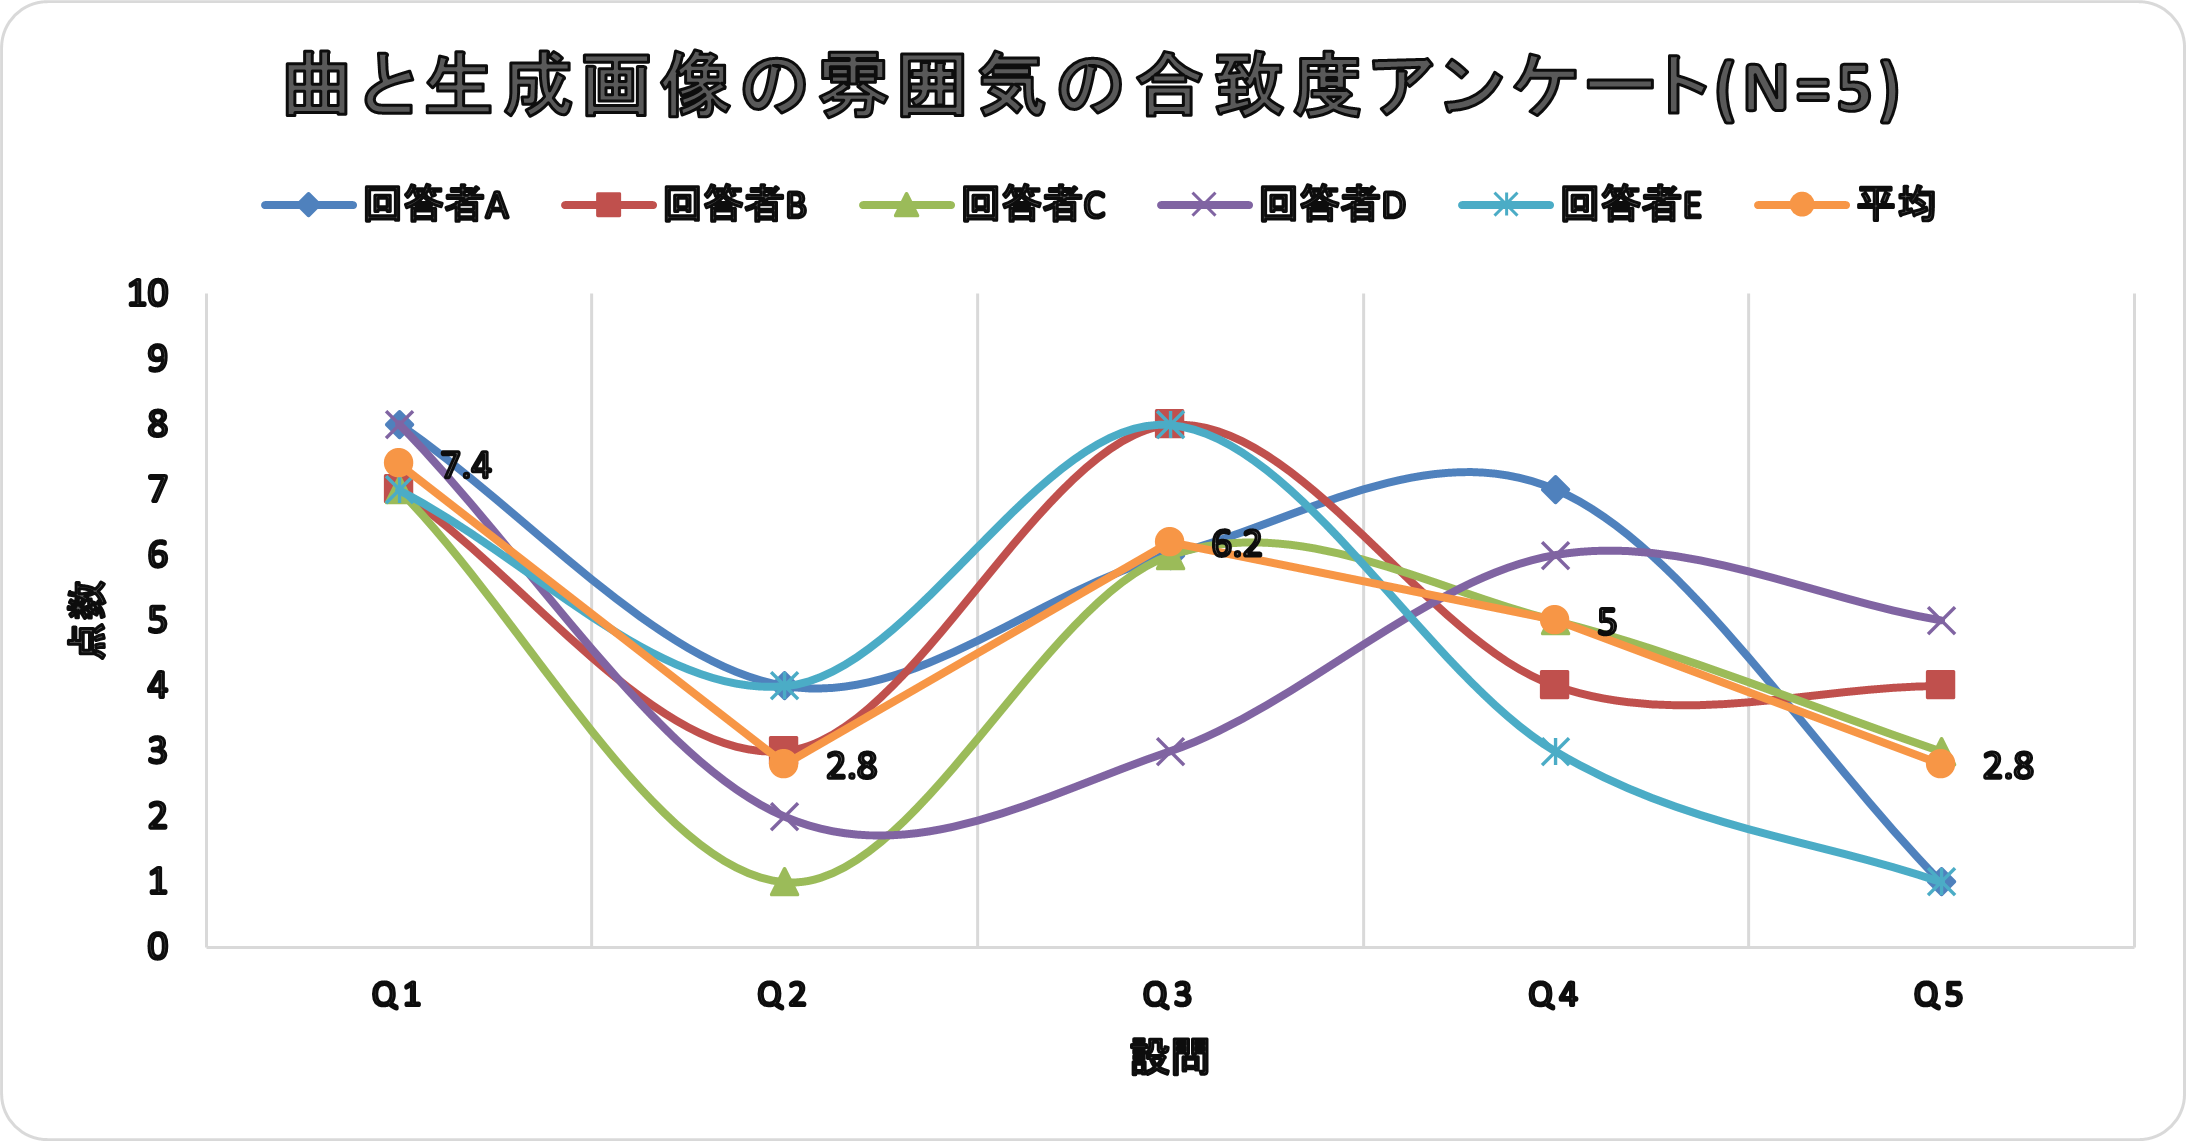
\includegraphics[width=0.85\textwidth]{./画像/アンケートグラフ.png}
  \caption{アンケート結果の集計グラフ}
  \label{fig:questionnaire_results}
\end{figure}

図\ref{fig:questionnaire_results}より,
回答者平均が中立値である 5 を約 1.2 ポイント下回る設問（Q2, Q5）,
中立値とほぼ一致する設問（Q3）,
および中立値を約 1.2 から 2.4 ポイント上回る設問（Q1, Q4）が確認された.
このことから, 音楽と生成画像の雰囲気の合致度には設問間でばらつきが存在することが分かる.

また, 表\ref{tab:similarity_matrix}に, 図\ref{fig:questionnaire_results}の各回答者間の評価結果の相関行列を示す.

\begin{table}[htbp]
\centering
\caption{回答者間の類似度行列}
\label{tab:similarity_matrix}
\begin{tabular}{c|ccccc}
\hline
 & 回答者A & 回答者B & 回答者C & 回答者D & 回答者E \\
\hline
回答者A & 1 &  &  &  &  \\
回答者B & 0.5319 & 1 &  &  &  \\
回答者C & 0.7332 & 0.8427 & 1 &  &  \\
回答者D & 0.4604 & 0.2512 & 0.6696 & 1 &  \\
回答者E & 0.7005 & 0.8566 & 0.6414 & 0.0218 & 1 \\
\hline
\end{tabular}
\end{table}

表\ref{tab:similarity_matrix}より, 
回答者Bと回答者C, 回答者Bと回答者Eの間で高い, 音楽と生成画像の雰囲気の合致度の感じ方の類似が確認できる一方, 
回答者Dと回答者Eの間では極めて低く, 被験者間で個人差が存在することが示唆される.
しかし, 相関係数は全て正の値であったため, 音楽と生成画像間の共通情報の取得の類似性を認められると確認した.

\newpage
\section{考察} 

% 本研究について,客観的な評価・考察を行う.
本研究により, 音楽から抽出した音響特徴量を基に単語ラベルを生成し, 
それを用いて画像生成AIによる視覚的イメージの生成が可能であることが確認された, 
また, アンケート結果から, 一部の楽曲においては, 
音楽と生成画像の雰囲気がある程度一致していると評価される例も見られ, 
本手法が音楽と視覚表現を結び付ける手段として一定の有効性を持つことが示唆された.
一方で, 評価結果全体を見ると, 設問間で合致度にばらつきが存在し, 
必ずしも安定して高い一致度が得られたとは言い難い. 
この要因として, いくつかの課題が考えられる. 

第一に, 学習に用いたデータセット数および生成ラベル数の不足が挙げられる.
GTZAN データセットはジャンル分類用途としては広く利用されているものの, 
音楽の雰囲気や情景を表す単語生成を目的とした場合には, 
必ずしも十分な多様性を持つとは限らない可能性がある.
また，単語ラベルの種類や数が限定的であったため, 
音楽が持つ複雑な印象を十分に表現しきれなかったと考えられる.

第二に, 学習データセット作成および単語ラベル設定における属人性の影響が考えられる. 
本研究では, 単語ラベルの定義や意味付けを筆者の主観に基づいて行っており, 
これがモデルの学習結果や生成画像に反映された可能性がある.
アンケートにおいて被験者間で評価の相関に差が見られた点も, 
音楽の捉え方や視覚的イメージの想起に個人差が存在することを示している.

第三に, 音楽と画像という異なる情報媒体間の本質的な差異も ,
合致度が十分に高まらなかった要因の一つと考えられる. 
音楽は時間的に変化する聴覚情報であるのに対し ,
画像は空間的に固定された視覚情報であり,
両者の情報量や表現内容は大きく異なる. 
このため, 音楽の印象を単語へ変換し, 
さらに画像へと対応付ける過程において,
情報の欠落や解釈のずれが生じやすかったと推察される.

以上より, 本研究で提案した手法は, 
音楽から画像生成を行う試みとして一定の可能性を示した一方で, 
データセットの拡充, ラベル設計の客観化, 
および個人差を考慮したモデル設計など, 
今後解決すべき課題が多く残されていることが明らかとなった.


\newpage 
\section{結論}

% 本研究で何を明らかにしたのか,また,
% 今後の課題としてどのような問題があるのか,
% といったことをまとめる.

\newpage 
\section{付録}

% プログラムや実行結果など,
% 本論を補足する上で必要と思われるものがあれば付録としてつける
% （なければつけなくてよい）.
単語ラベルは以下のカテゴリに分類される．
\begin{itemize}
  \item 形容詞（音の印象）：
  明るい，暗く寂しい，静か・滑らか，激しい・力強い，
  幻想的・夢幻的，高貴・荘厳，現代的，情熱的

  \item 名詞（音から想起される情景）：
  自然風景，都市・人工物，時間・空模様，抽象・感情，神秘的な場所

  \item 動作表現：
  鳴り響くように

  \item 季節：
  春，夏，秋，冬

  \item 色：
  赤，橙，黄，黄緑，緑，水色，青，紫，
  ピンク，茶色，黒，白
\end{itemize}


\newpage 
%% 参考文献

\begin{thebibliography}{}

\bibitem{中山} 中山 達喜, 吉田 真一 ：音楽分類における特徴量の検討，
\url{https://www.jstage.jst.go.jp/article/fss/26/0/26_0_290/_article/-char/ja/}
 (2010). 

\bibitem{Xiaoli} Xiaoli Chu : Feature Extraction and Intelligent Text Generation of Digital Music,
https://pubmed.ncbi.nlm.nih.gov/35845909/
 (2020).

\bibitem{Tzanetakis} G. Tzanetakis; P. Cook : Musical genre classification of audio signals,
https://ieeexplore.ieee.org/abstract/document/1021072
 (2002).

\bibitem{Meyers} Meyers, Owen Craigie : A mood-based music classification and exploration system,
https://dspace.mit.edu/handle/1721.1/39337
 (2007).

\bibitem{Ledge} Ledge.ai 編集部 ：教師なし学習とは | 教師あり学習や強化学習との違い・活用事例・代表的なアルゴリズムを紹介，
https://ledge.ai/articles/unsupervised
 (2020).

\end{thebibliography}


\end{document}